\section{Анализ электронных писем Хиллари Клинтон}

\subsection{Длины слов и писем}

\begin{itemize}

\item На основании содержаний писем можно посчитать различные статистики, например,
распределение длин слов по письмам: 

\begin{figure}[H]
\centering
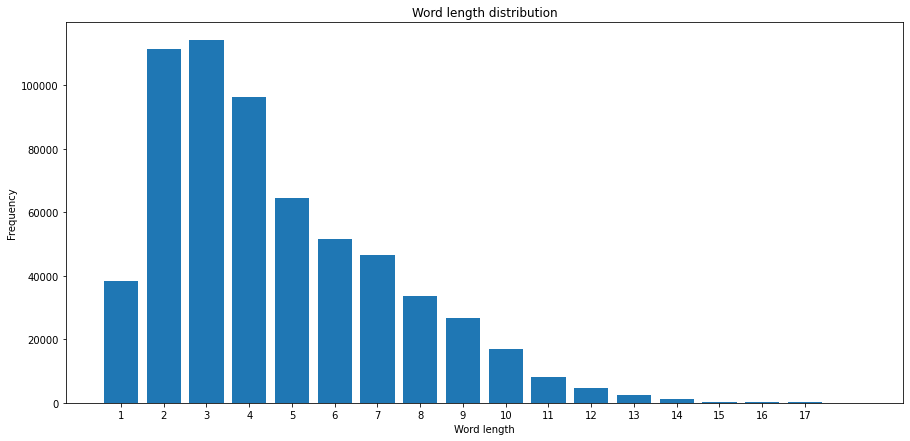
\includegraphics[scale=0.5]{pics/word_lengths.png}
\caption{Гистограмма распределения длин слов в наборе Клинтон}
\end{figure}


Гистограмма выглядит вполне естественным образом, много коротких слов, что естественно для английского языка.

\item Аналогично мы можем посчитать распределения длин писем (по количеству слов):

\begin{figure}[H]
\centering
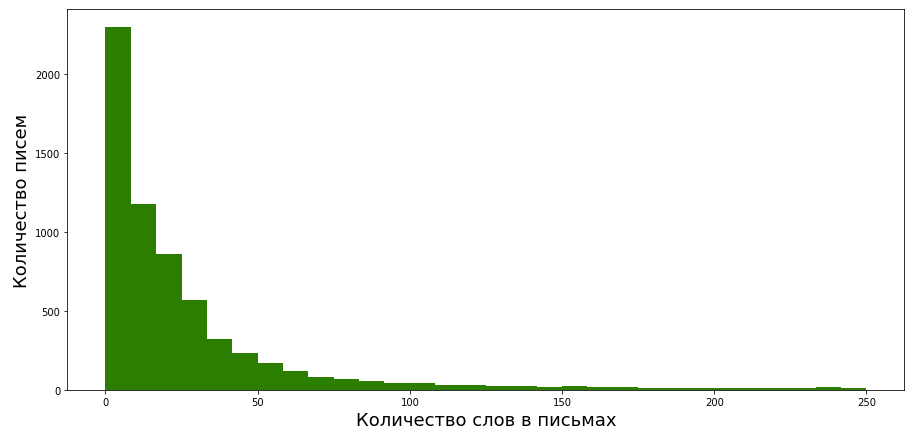
\includegraphics[scale=0.5]{pics/email_lengths.png}
\caption{Распределение количества слов в письмах в наборе Клинтон}
\end{figure}

Гистограмма соответствует интуитивным ожиданиям -- более длинные письма пишутся реже. 
\end{itemize}

\subsection{Время отправки писем}


\begin{itemize}

\item В метаданных писем содержится информация об дате отправки писем, на основании этого
можно проанализировать, например, в какие года были отправлены письма:


\begin{figure}[H]
\centering
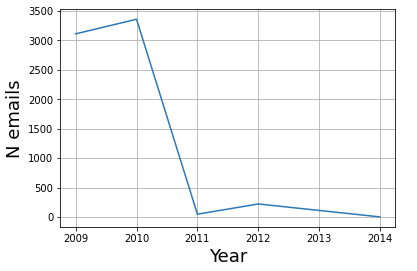
\includegraphics[scale=0.8]{pics/year.png}
\caption{График количества отправленных писем по годам в наборе Клинтон}
\end{figure}

На графике можно заметить странную аномалию с нулем писем в 2011 году. Вероятнее всего, это связано с особенностями набора данных. 

\item Аналогично можно проанализировать дни недели отправки писем:

\begin{figure}[H]
\centering
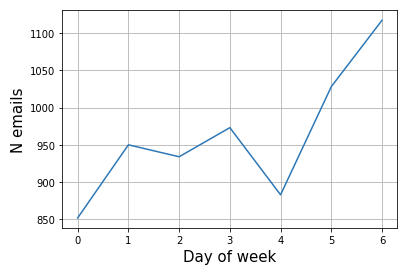
\includegraphics[scale=0.8]{pics/week.png}
\caption{График количества отправленных писем по дням недели в наборе Клинтон}
\end{figure}


График выглядит слегка неестественно (в отличие от \textit{Enron}). Можно попытаться интерпретировать это как особенности одного отдельного человека, занимающего специфичным видом деятельности.

 
\end{itemize}
